
\chapter{Introduzione}
L'obiettivo del progetto realizzato è quello di integrare la libreria Orocos KDL (\url{https://www.orocos.org/kdl.html}) nel component framework \textit{STAR} per lo sviluppo di un'applicazione che consente di inviare dei comandi di movimento ai motori di un robot manipolatore affinché l'end-effector raggiunga una particolare posizione finale, espressa nel sistema di riferimento della base del robot, seguendo un percorso lineare. Il robot manipolatore utilizzato è il modello P-Rob 3, prodotto dalla F\&P Personal Robotics (\Fig\ref{fig:prob3}). 
\begin{figure}[b!]
	\centering
	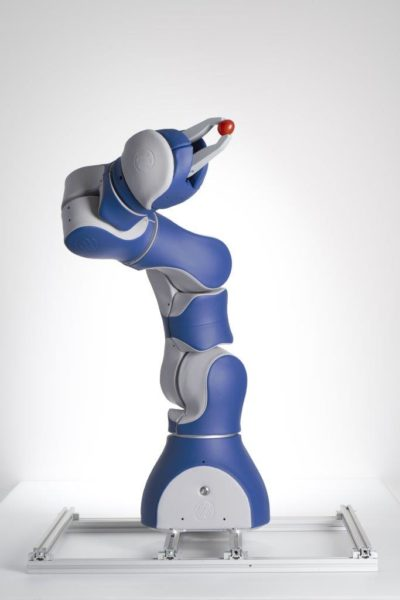
\includegraphics[width=0.4\linewidth]{./ImageFiles/P-Rob 3.jpg}
	\caption{Robot manipolatore P-Rob 3.}
	\label{fig:prob3}
\end{figure}
In particolare, sono state sviluppate le seguenti funzionalità:
\begin{itemize}
	\item calcolo della posizione della pinza espressa nel sistema di riferimento della base del robot a partire dal valore degli angoli dei giunti (cinematica diretta);
	\item calcolo del valore dei giunti a partire dalla posizione della pinza espressa nel sistema di riferimento della base del robot (cinematica inversa);
	\item calcolo di un percorso lineare a partire da una posizione iniziale e una finale della pinza espresse nel sistema di riferimento della base del robot.
\end{itemize}

\chapter{Libreria Orocos KDL}
\section{Installazione}
Per effettuare i calcoli cinematici si è scelto di utilizzare la libreria Orocos KDL che implementa alcuni algoritmi, come il calcolo della cinematica diretta e inversa, per un robot opportunamente descritto da un file di configurazione. Seguendo la guida di installazione disponibile nella documentazione (\url{https://www.orocos.org/wiki/Installation_Manual.html}), la libreria è stata installata nel framework \textit{STAR} al seguente percorso: \\ 
\centerline{\texttt{STAR/AutonomousRobot/Libraries/others/orocos\_kinematics\_dynamics.}} \\
Inoltre, per semplificare alcune operazioni di inizializzazione degli oggetti utilizzati dalla libreria Orocos KDL, è stata installata anche la libreria \textit{KDL Parser} (\url{https://github.com/ros/kdl_parser}) nella cartella \\ \centerline{\texttt{STAR/AutonomousRobot/Libraries/others/kdl\_parser}.} \\ Infine, è stato modificato il file \textit{env-star.sh} inserendo le informazioni per includere i file e recuperare i binari delle librerie installate necessari alla compilazione dei componenti e plugin sviluppati.

\section{Definizione del modello del robot}
La libreria Orocos KDL ha bisogno di conoscere la struttura cinematica del robot. La catena cinematica del robot è stata definita in un file .urdf (\url{http://wiki.ros.org/urdf}), nel quale sono descritti in modo standard tutti i parametri, quali ad esempio il numero, la tipologia e i limiti dei giunti e le caratteristiche dei link. Per definire questo file, si è partiti dal modello fornito sulla pagina github del produttore (\url{https://github.com/fp-robotics/fp_descriptions}), generando il file urdf seguendo la procedura indicata in tale pagina. Successivamente, il file è stato modificato per estrapolare le informazioni rilevanti per il progetto e, eseguendo delle prove con l'interfaccia di controllo web del robot, sono stati verificati alcuni dati presenti nell'urdf. La catena cinematica descritta dall'urdf è riportata in figura \ref{fig:urdf_prob3}.
\begin{figure}[tbh]
	\centering
	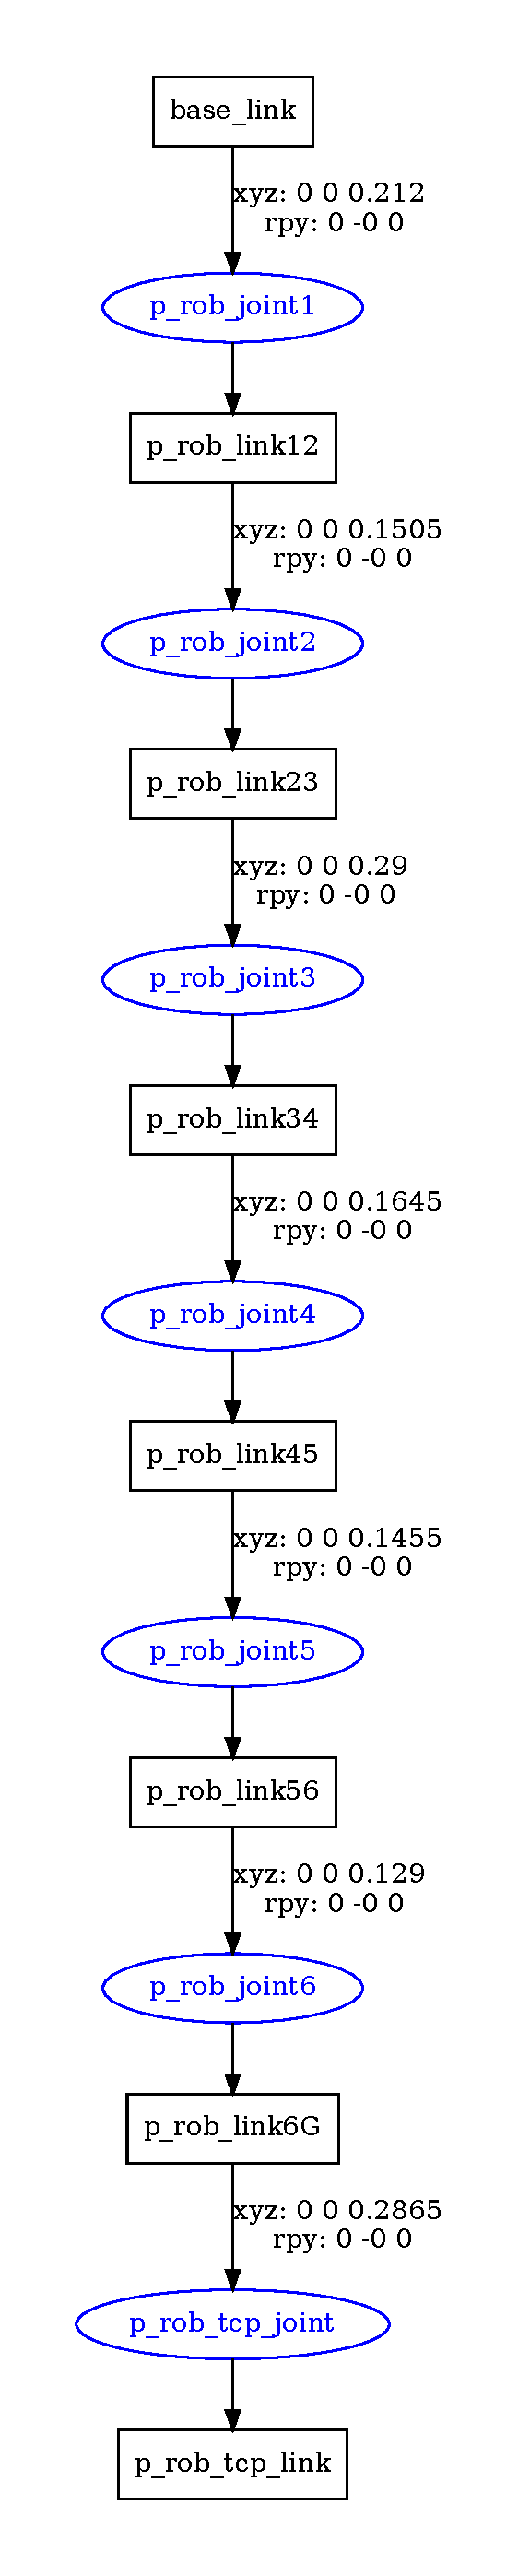
\includegraphics[width=0.3\linewidth]{./OtherFiles/p_rob.pdf}
	\caption{Catena cinematica descritta nel file urdf.}
	\label{fig:urdf_prob3}
\end{figure}
Nel file urdf, che è strutturato come un file xml, è possibile specificare i giunti e i link del robot tramite i seguenti elementi:
\begin{itemize}
	\item \tl link name="xxx"\tr...\tl /link\tr, elemento che descrive le caratteristiche di un link;
	\item \tl joint name="yyy" type="revolute"\tr...\tl /joint\tr, elemento che descrive le caratteristiche di un giunto; il robot utilizzato è costituito da sei giunti di rotazione, per cui il tipo dei giunti è definito come "revolute".
\end{itemize}
All'interno degli elementi è possibile poi specificare diverse caratteristiche tra le quali (elenco completo reperibile al link \url{http://wiki.ros.org/urdf/XML/joint}):
\begin{itemize}
	\item  \tl parent link="xxx"/\tr\ e \tl child link="yyy"/\tr\ indicano rispettivamente il link padre e il link figlio di un giunto;
	\item \tl axis xyz="0 1 0"/\tr\ indica l'asse di rotazione del giunto;
	\item  \tl origin xyz="x y z r p y"/\tr\ indica la rototraslazione tra il link padre e il link figlio (valori x, y, z espressi in metri e r, p ,y in radianti).
	\item \tl limit effort="1.09" lower="-2.949" upper="2.967" velocity="0.829"/\tr \ descrive i limiti di velocità, angolo massimo e minimo ed effort di un giunto;
\end{itemize}
Per descrivere il robot utilizzato sono quindi stati definiti sei giunti di rotazione (tre con asse di rotazione lungo l'asse z e tre con asse di rotazione lungo l'asse y) e sette link dalla base del robot fino al centro di presa. Sono stati poi aggiunti un giunto di tipo \textit{fisso} e un link terminale per rappresentare correttamente il centro di presa.

\clearpage

\section{KDL Paser} \label{cap_kdlparser}
A partire dalla descrizione del robot contenuta nel file urdf, è necessario costruire una struttura dati di tipo \texttt{KDL::Chain}, utilizzata dalla libreria Orocos KDL per i calcoli cinematici. Per fare ciò, si è utilizzato la libreria KDL Parser. Inizialmente, viene eseguito il parsing del file urdf tramite la funzione \texttt{urdf::parseURDFFile(path\_urdf)} che restituisce un oggetto di tipo \texttt{urdf::ModelInterfaceSharedPtr} che rappresenta il modello del file urdf. Se questa operazione viene effettuata correttamente, l'oggetto appena creato viene utilizzato per generare un oggetto di tipo \texttt{KDL::Tree} tramite la funzione \texttt{kdl\_parser::treeFromUrdfModel} che rappresenta la struttura del robot. Se l'oggetto viene creato correttamente, si utilizza il metodo \texttt{my\_tree.getChain("base\_link", "last\_link", m\_chain)} per definire un oggetto di tipo \texttt{KDL::Chain} che rappresenta la catena cinematica del robot dal link "base\_link", il cui nome viene specificato come primo parametro della funzione, fino al link finale "last\_link", specificato come secondo parametro e che corrisponde al centro di presa. Un oggetto di tipo \texttt{KDL::Chain} è costituito da \texttt{KDL::Segment}, dove un segmento rappresenta un link con un giunto e con due collegamenti alle estremità con altri segmenti. 
Successivamente, dall'oggetto \texttt{KDL::Chain} vengono estratti i limiti dei giunti (in termini di angoli minimi e massimi raggiungibili dai giunti). Essi vengono salvati in un array di tipo \texttt{KDL::JntArray} e saranno utilizzati nel calcolo della cinematica inversa.

\section{Sistemi di riferimento del robot}
Nelle figure \ref{fig:base_frame} e \ref{fig:tool_frame} sono riportati i sistemi di riferimento rispetto alla base del robot e del tool che sono stati considerati nel progetto. Inoltre le convenzioni scelte per indicare le rotazioni prevedono che gli angoli di roll (\textalpha), pitch (\textbeta) e yaw (\textgamma) siano definiti rispetto alla terna fissa (x,y,z) della base del robot, eseguendo le rotazioni nel seguente ordine: rotazione attorno all'asse x di angolo \textalpha, rotazione attorno all'asse y di angolo \textbeta\ e rotazione attorno all'asse z di angolo \textgamma.

\begin{figure}[tbh]
	\centering
	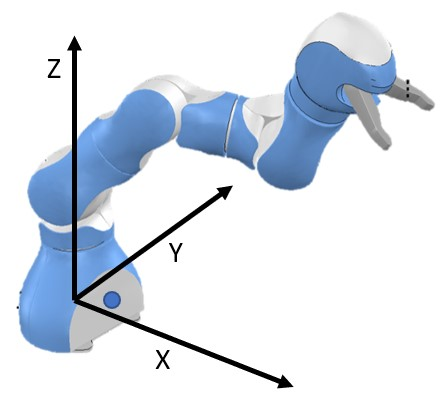
\includegraphics[width=0.5\linewidth]{./ImageFiles/prob_frame_base}
	\caption{Sistema di riferimento alla base del robot.}
	\label{fig:base_frame}
\end{figure}

\begin{figure}[tbh]
	\centering
	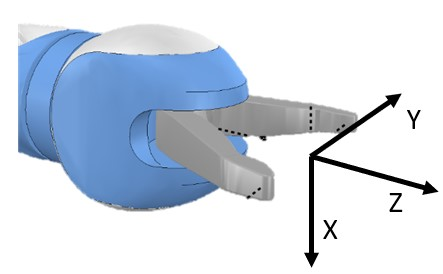
\includegraphics[width=0.5\linewidth]{./ImageFiles/prob_frame_tool.jpg}
	\caption{Sistema di riferimento del tool.}
	\label{fig:tool_frame}
\end{figure}

\clearpage

\section{Cinematica diretta} \label{cap_fk}
La cinematica diretta permette di calcolare la posizione e l'orientamento dell'end-effector a partire dal valore dei giunti. La libreria Orocos KDL mette a disposizione il metodo \\ \centerline{\texttt{int KDL::ChainFkSolverPos\_recursive::JntToCart(const JntArray\& q\_in, Frame\& p\_out)}} \\ che riceve in ingresso un vettore \textit{q\_in} di tipo \texttt{KDL::JntArray} che contiene la configurazione dei giunti e restituisce la posizione dell'end-effector rispetto al sistema del riferimento della base tramite l'oggetto \textit{p\_out} di tipo \texttt{KDL::Frame}, che rappresenta una rototraslazione nello spazio 3D. Il valore intero restituito indica l'esito del calcolo della cinematica diretta (zero se il calcolo è stato effettuato con successo). Questo metodo appartiene alla classe \texttt{KDL::ChainFkSolverPos\_recursive} che implementa un algoritmo ricorsivo per il calcolo della cinematica diretta. Il costruttore di questa classe \\ \centerline{\texttt{ChainFkSolverPos\_recursive (const Chain \&chain)}} \\ richiede come parametro un oggetto \texttt{KDL::Chain}.

\section{Cinematica inversa} \label{cap_ik}
La cinematica inversa permette di calcolare la configurazione dei giunti a partire dalla posizione dell'end-effector espressa nel sistema di riferimento della base. La libreria Orocos 
KDL mette a disposizione diversi risolutori che implementano differenti algoritmi per il calcolo della cinematica inversa tramite metodi iterativi. In questo progetto è stato utilizzato il risolutore \texttt{KDL::ChainIkSolverPos\_NR\_JL} che implementa un metodo generale per la risoluzione della cinematica inversa utilizzando il metodo di Newton-Raphson tenendo in considerazione i limiti dei giunti. Il costruttore del risolutore ha la seguente segnatura: \\ \texttt{KDL::ChainIkSolverPos\_NR\_JL::ChainIkSolverPos\_NR\_JL(const Chain \&\ chain, const JntArray \&\ q\_min, const JntArray \&\ q\_max, ChainFkSolverPos \&\ fksolver, \\ ChainIkSolverVel \&\ iksolver, unsigned int	maxiter = 100, double eps = 1e-6)}, \\ dove \textit{chain} è un oggetto di tipo \texttt{KDL::Chain} che corrisponde alla descrizione della catena cinematica del robot, \textit{q\_min} e \textit{q\_max} contengono i limiti dei giunti, \textit{fksolver} rappresenta un riferimento a un risolutore di cinematica diretta, \textit{iksolver} un riferimento a un risolutore di cinematica inversa differenziale (nel progetto è stato utilizzato un risolutore di tipo\texttt{ KDL::ChainIkSolverVel\_pinv}), \textit{maxiter} rappresenta il numero massimo di iterazioni e \textit{eps} rappresenta il massimo errore espresso in metri della posizione raggiunta dall'end-effector con i valori degli angoli ottenuti rispetto alla posizione richiesta. Nel progetto sono stati scelti un numero di iterazione massimo pari a 1000 e una precisione di \SI{1}{\milli\meter}. 
La classe \texttt{KDL::ChainIkSolverPos\_NR\_JL} fornisce il metodo \\
\texttt{int KDL::ChainIkSolverPos\_NR\_JL::CartToJnt(const JntArray \&\ q\_init, const Frame \&\ p\_in, JntArray \&\	q\_out)} \\ che, data la posizione dell'end-effector tramite il parametro \textit{p\_in}, restituisce i valori dei giunti calcolati nella variabile \textit{q\_out}. Il parametro \textit{q\_init} rappresenta la configurazione iniziale dei giunti dalla quale il metodo iterativo inizia la ricerca della soluzione della cinematica inversa e può influenzare la configurazione finale dei giunti. Il valore intero restituito indica l'esito dell'operazione (zero se il calcolo è andato a buon fine).

\section{Traiettoria lineare} \label{cap_lt}
La classe \texttt{KDL::Path\_Line}, che estende \texttt{KDL::Path}, permette di creare un oggetto che rappresenta un percorso lineare da una posizione iniziale ad una finale. Di seguito si riporta il costruttore di un oggetto di tipo \texttt{KDL::Path\_Line}: \\ \texttt{Path\_Line (const Frame \&F\_base\_start, const Frame \&F\_base\_end, RotationalInterpolation *orient, double eqradius, bool \_aggregate=true)}.\\ I parametri \texttt{F\_base\_start} e \texttt{F\_base\_end} rappresentano i sistemi di riferimento della posizione iniziale e finale del percorso lineare che si vuole calcolare: in questo progetto coincidono con la posizione iniziale e finale dell'end-effector. Il parametro \textit{orient} di tipo \texttt{KDL::RotationalInterpolation} è utilizzato dalla classe per rappresentare la rotazione associata a un percorso geometrico. La documentazione della libreria suggerisce di inizializzare questo parametro attraverso il metodo \\ \centerline{\texttt{KDL::RotationalInterpolation\_SingleAxis()}} \\ che ha il vantaggio di essere indipendente dal sistema di riferimento nel quale si esprime il percorso. Il parametro \textit{eqradious} è di tipo \texttt{double} e rappresenta l'\textit{equivalent radious}. Questo parametro serve a comparare le rotazioni con le traslazioni, definendo la "quantità di movimento" di una rotazione come lo spazio percorso da un punto a distanza \textit{eqradious} dall'asse di rotazione. Nel progetto, si è scelto di assegnare a questo parametro il valore arbitrario 1. Tuttavia, sviluppi futuri richiederanno di approfondire il valore ottimo da assegnare a questo parametro.
Per il progetto sono stati utilizzati anche i seguenti metodi della classe \texttt{KDL::Path\_Line}:
\begin{itemize}
	\item \texttt{double KDL::Path\_Line::PathLength()}: restituisce la lunghezza del percorso. Tuttavia, la lunghezza restituita non è da considerarsi sempre come una lunghezza fisica, ad esempio quando la componente di rotazione è dominante;
	\item \texttt{Frame KDL::Path\_Line::Pos(double s)}: ritorna il sistema di riferimento lungo il percorso alla lunghezza \textit{s} attuale. Questo metodo permette di ricavare i \textit{waypoints} all'interno del percorso lineare.
\end{itemize}

\chapter{Implementazione in STAR}
In figura \ref{fig:star_diagram} è riportato il diagramma dei componenti inseriti nel framework STAR. 
\begin{figure}[tbh]
	\centering
	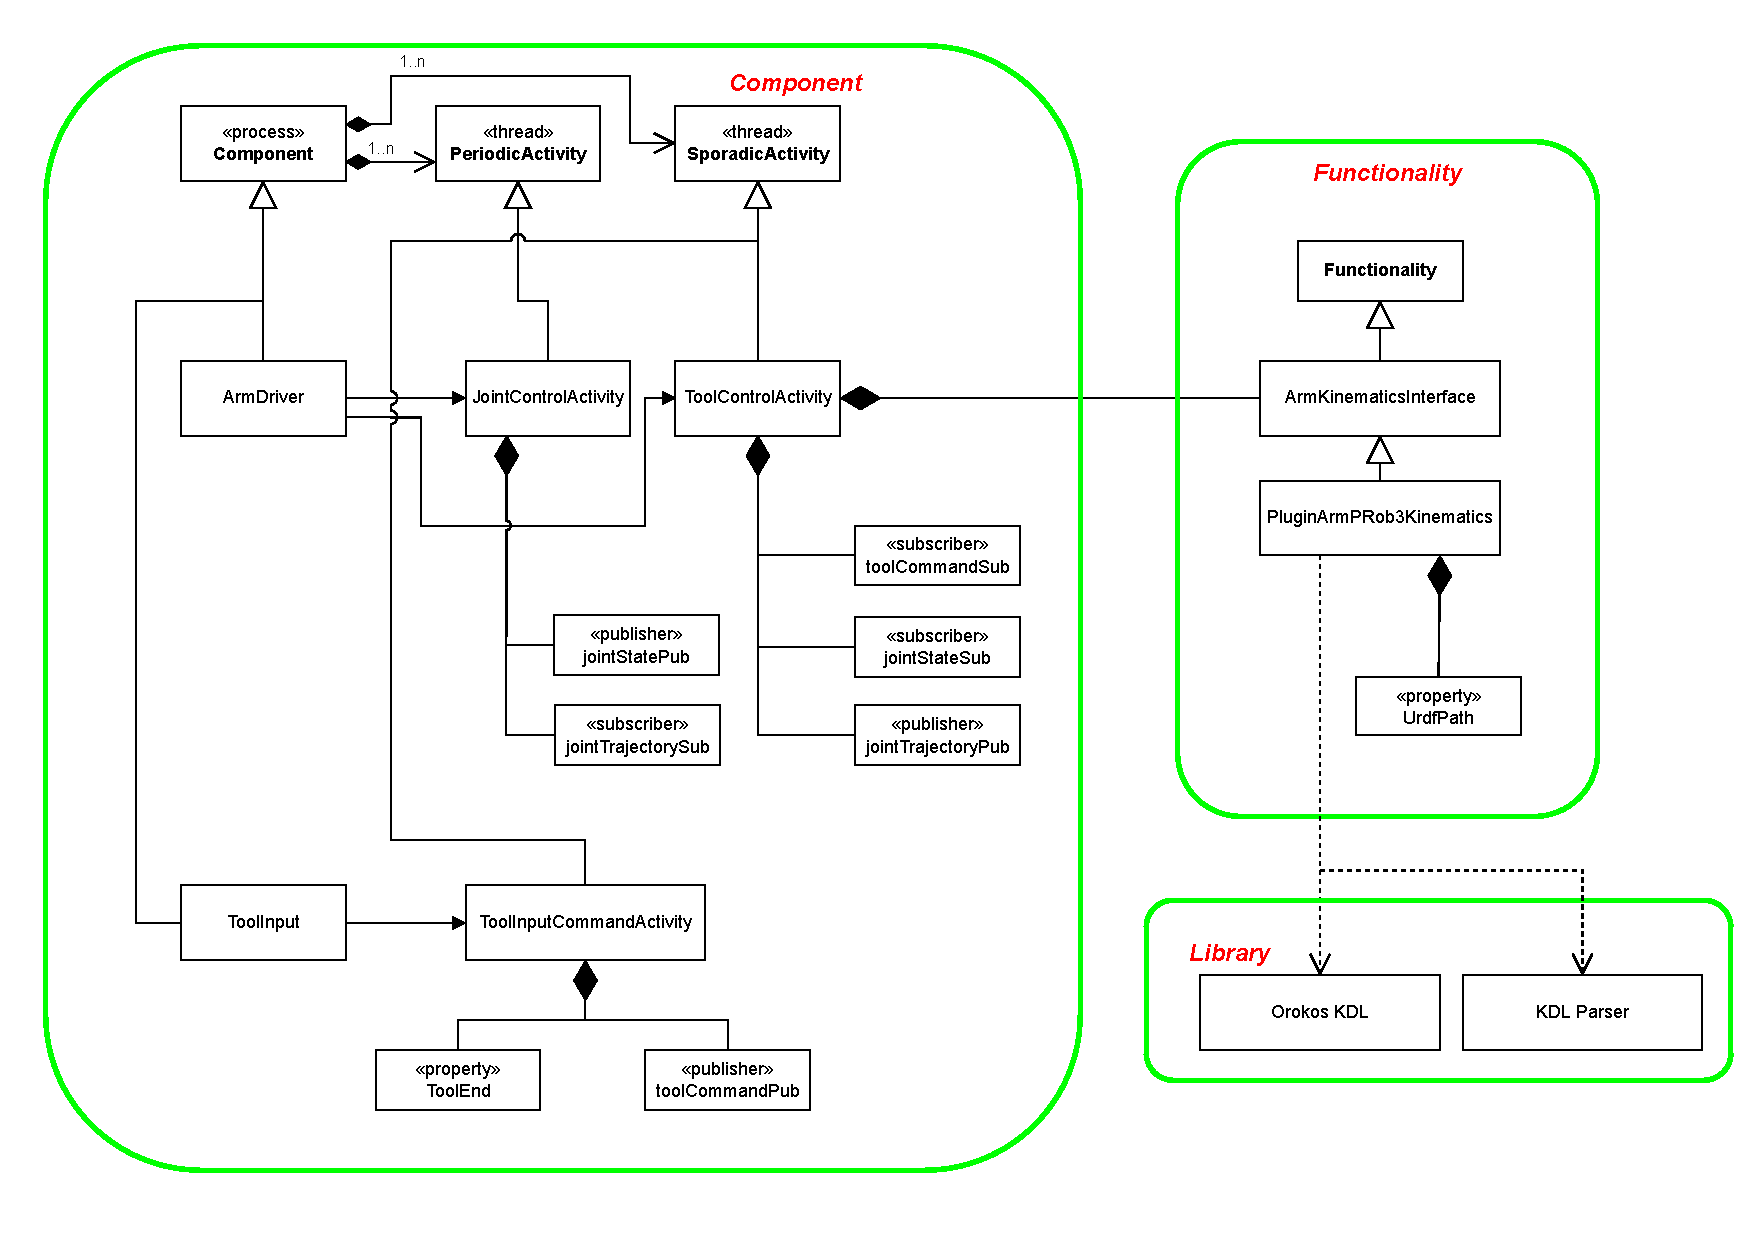
\includegraphics[width=1\linewidth]{./ImageFiles/publish_subscribe_architecture.drawio.pdf}
	\caption{Diagramma dei componenti STAR.}
	\label{fig:star_diagram}
\end{figure}

\noindent
Sono stati sviluppati due \textit{Component}:
\begin{itemize}
	\item \textit{ArmDriver}: implementa l'attività \textit{JointControlActivity} che si occupa di comunicare con il robot inviandogli i comandi di movimento e ricevendo la posizione corrente dei giunti, e la \textit{ToolControlActivity} che si occupa di elaborare la traiettoria lineare che l'end-effector dovrà seguire. 
	\item \textit{ToolInput}: implementa l'attività \textit{ToolInputCommandActivity} che si occupa di inviare la posizione target che il tool deve raggiungere a partire dalla posizione corrente.
\end{itemize}
\noindent
L'attività \textit{ToolControlActivity} utilizza le funzionalità della classe \textit{PluginArmPRob3Kinematics}, la quale fornisce le funzioni per eseguire la cinematica diretta, la cinematica inversa ed il calcolo di un percorso lineare utilizzando la libreria Orocos KDL.

\section{Plugin: PluginArmPRob3Kinematics}
Il plugin \textit{PluginArmPRob3Kinematics} implementa l'interfaccia \textit{ArmKinematicsInterface} e fornisce le funzionalità per il calcolo della cinematica diretta, della cinematica inversa e per la computazione di un percorso lineare. Per fare ciò utilizza le funzioni della libreria Orocos KDL descritte nella sezione precedente. 
In figura \ref{fig:plugin_uml} è riportato il diagramma della classe in questione.
\begin{figure}[ht!]
	\centering
	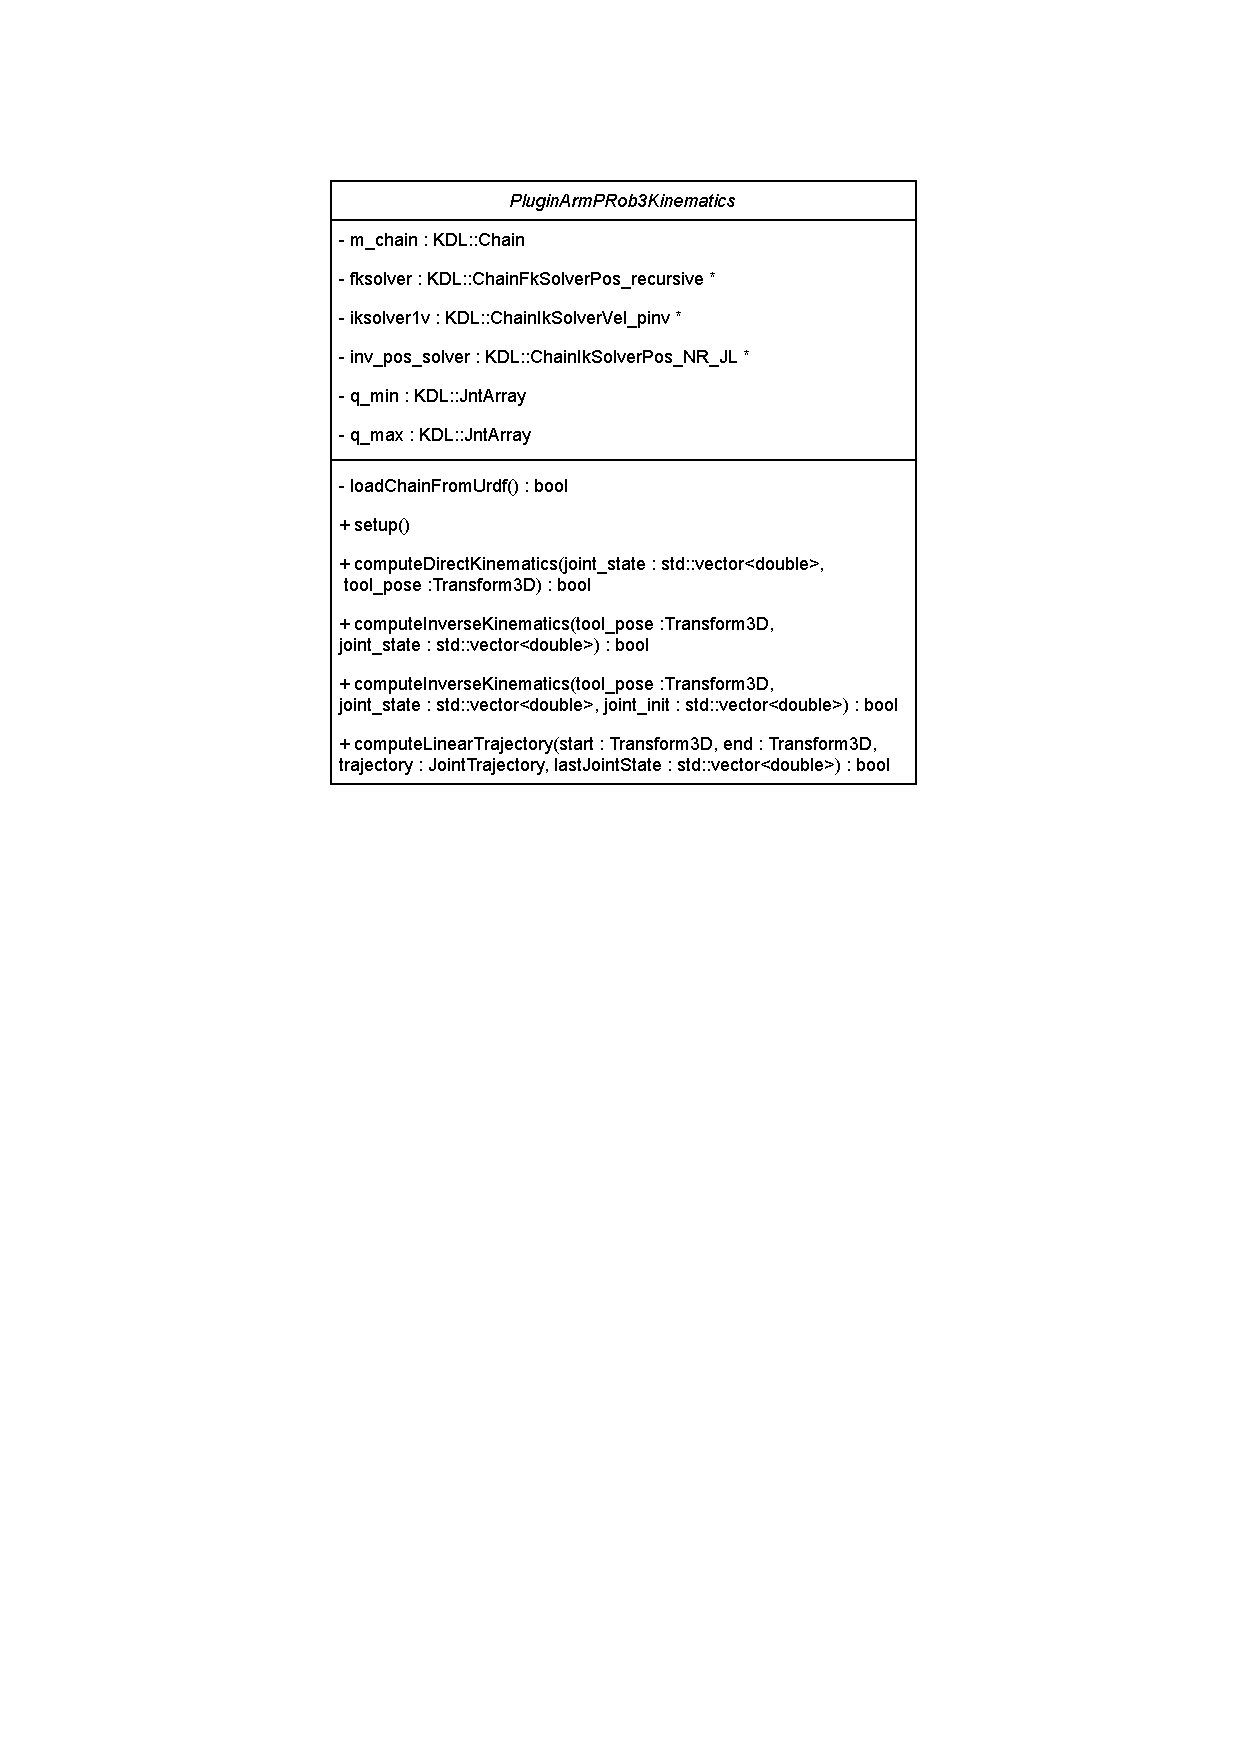
\includegraphics[width=0.5\linewidth]{./ImageFiles/PluginArmPRob3Kinematics.drawio.pdf}
	\caption{Diagramma UML della classe \texttt{PluginArmPRob3Kinematics}.}
	\label{fig:plugin_uml}
\end{figure}

\paragraph{VProperty\tl std::string\tr urdf}
Campo che rappresenta il nome del file urdf da utilizzare. Il file deve essere presente al seguente path: \\
\centerline{\texttt{AutonomousRobots/Functionalities/plugins/arm\_prob3\_kinematics/cfg}.}

\paragraph{KDL::Chain m\_chain}
Oggetto che incapsula la catena cinematica del robot.

\paragraph{KDL::JntArray q\_min, q\_max}
Rappresentano i limiti inferiori e superiori dei valori degli angoli dei giunti del robot. Vengono estratti dall'urdf quando viene chiamata la funzione \texttt{loadChainFromUrdf()}.

\paragraph{bool loadChainFromUrdf()}
Funzione che si occupa di estrarre la \texttt{KDL::Chain} ed i limiti dei giunti a partire dall'urdf del robot attraverso le funzioni fornite dalla libreria KDL Parser descritte nella sezione precedente (cap.\ref{cap_kdlparser}).\\
\textbf{\textit{Return:}}
\begin{itemize}
	\item \texttt{true}: se è stato estratto un oggetto \texttt{KDL::Chain} dall'urdf;
	\item \texttt{false}: altrimenti.
\end{itemize}

\paragraph{void setup()}
Metodo in cui vengono inizializzati tutti gli oggetti necessari al funzionamento del plugin. In particolare, vengono inizializzate le classi della libreria Orocos KDL necessarie al calcolo della cinematica diretta ed inversa e viene letto l'urdf tramite il metodo \texttt{loadChainFromUrdf()}.

\paragraph{bool computeDirectKinematics(std::vector\tl double\tr \&joint\_state, Transform3D \&toolPose)}
Metodo che si occupa di eseguire il calcolo della cinematica diretta utilizzando la funzione \texttt{KDL::ChainFkSolverPos\_recursive::JntToCart(const JntArray \&q\_in, Frame \&q\_out)} (cap.\ref{cap_fk}).\\
\textbf{\textit{Parametri:}}
\begin{itemize}
	\item \texttt{joint\_state}: input, valore dei giunti da cui si vuole calcolare la posizione dell'end-effector; 
	\item \texttt{toolPose}: output, oggetto che rappresenta la posizione dell'end-effector rispetto alla base del robot.
\end{itemize}
\textbf{\textit{Return:}}
\begin{itemize}
	\item \texttt{true}: la cinematica diretta è stata calcolata senza errori;
	\item \texttt{false}: altrimenti.
\end{itemize}


\paragraph{bool computeInverseKinematics(Transform3D \&tool\_pose, std::vector\tl double\tr \&joint\_state)}
Metodo che si occupa di eseguire il calcolo della cinematica inversa utilizzando la funzione \\ \texttt{ChainIkSolverPos\_NR\_JL::CartToJnt(const JntArray \&q\_init, const Frame \&p\_in, \\ JntArray \&q\_out)} (cap.\ref{cap_ik}). \\In questo caso, il valore iniziale dei giunti da cui si parte a calcolare la soluzione della cinematica inversa (parametro \textit{q\_init}) è pari a 0, che corrisponde alla posizione del robot P-Rob 3 completamente disteso con la pinza rivolta verso l'alto.\\
\textbf{\textit{Parametri:}}
\begin{itemize}
	\item \texttt{toolPose}: input, oggetto che rappresenta la posizione dell'end-effector rispetto alla base del robot di cui si vogliono conoscere i rispettivi valori dei giunti;
	\item \texttt{joint\_state}: output, valore dei giunti associati alla posizione dell'end-effector rappresentata da \texttt{toolPose}.
\end{itemize}
\textbf{\textit{Return:}}
\begin{itemize}
	\item \texttt{true}: la cinematica inversa è stata calcolata senza errori;
	\item \texttt{false}: altrimenti.
\end{itemize}

\paragraph{bool computeInverseKinematics(Transform3D \&tool\_pose, std::vector\tl double\tr \&joint\_state, std::vector\tl double\tr \&joint\_init)}
Metodo che si occupa di eseguire il calcolo della cinematica inversa utilizzando la funzione \texttt{ChainIkSolverPos\_NR\_JL::CartToJnt(const JntArray \&q\_init, const Frame \&p\_in, JntArray \&q\_out)} (cap.\ref{cap_ik}). A differenza del metodo precedente, è possibile specificare la posizione iniziale dei giunti del robot da cui si parte a calcolare la cinematica inversa. \\
\textbf{\textit{Parametri:}}
\begin{itemize}
	\item \texttt{toolPose}: input, oggetto che rappresenta la posizione dell'end-effector rispetto alla base del robot di cui si vogliono conoscere i valori dei giunti;
	\item \texttt{joint\_state}: output, valore dei giunti associati alla posizione dell'end-effector.
	\item \texttt{joint\_init}: input, valore iniziale dei giunti da cui partire per il calcolo della cinematica inversa con metodi incrementali.
\end{itemize}
\textbf{\textit{Return:}}
\begin{itemize}
	\item \texttt{true}: la cinematica inversa è stata calcolata senza errori;
	\item \texttt{false}: altrimenti.
\end{itemize}


\paragraph{bool computeLinearTrajectory(Transform3D \&start, Transform3D \&end, JointTrajectory \&trajectory, std::vector\tl double\tr \&lastJointState)}
Metodo tramite cui è possibile computare, a partire da un punto iniziale ed un punto finale nello spazio, un percorso lineare che l'end-effector dovrà seguire (cap.\ref{cap_fk}). In figura \ref{fig:algorithm} è mostrato il funzionamento dell'algoritmo che computa il percorso lineare. Si osservi che, nel caso in cui non la cinematica inversa non venga calcolata correttamente per un punto lungo il percorso, l'algoritmo riparte dall'inizio perturbando in modo incrementale il valore iniziale dei giunti nel calcolo del primo \textit{waypoint} della traiettoria. \\
\textbf{\textit{Parametri:}}
\begin{itemize}
	\item \texttt{start}: input, oggetto che rappresenta la posizione iniziale dell'end-effector;
	\item \texttt{end}: input, oggetto che rappresenta la posizione finale  che l'end-effector dovrà raggiungere seguendo un percorso lineare;
	\item \texttt{trajectory}: output, oggetto che contiene un array di valori dei giunti che rappresentano i punti di passaggio lungo la retta che il robot deve seguire;
	\item \texttt{lastJointState}: input, vettore contenente i valori dei giunti della posizione corrente del robot. 
\end{itemize}
\textbf{\textit{Return:}}
\begin{itemize}
	\item \texttt{true}: un percorso lineare è stata trovato senza errori;
	\item \texttt{false}: altrimenti.
\end{itemize}

\begin{figure}[ht!]
	\centering
	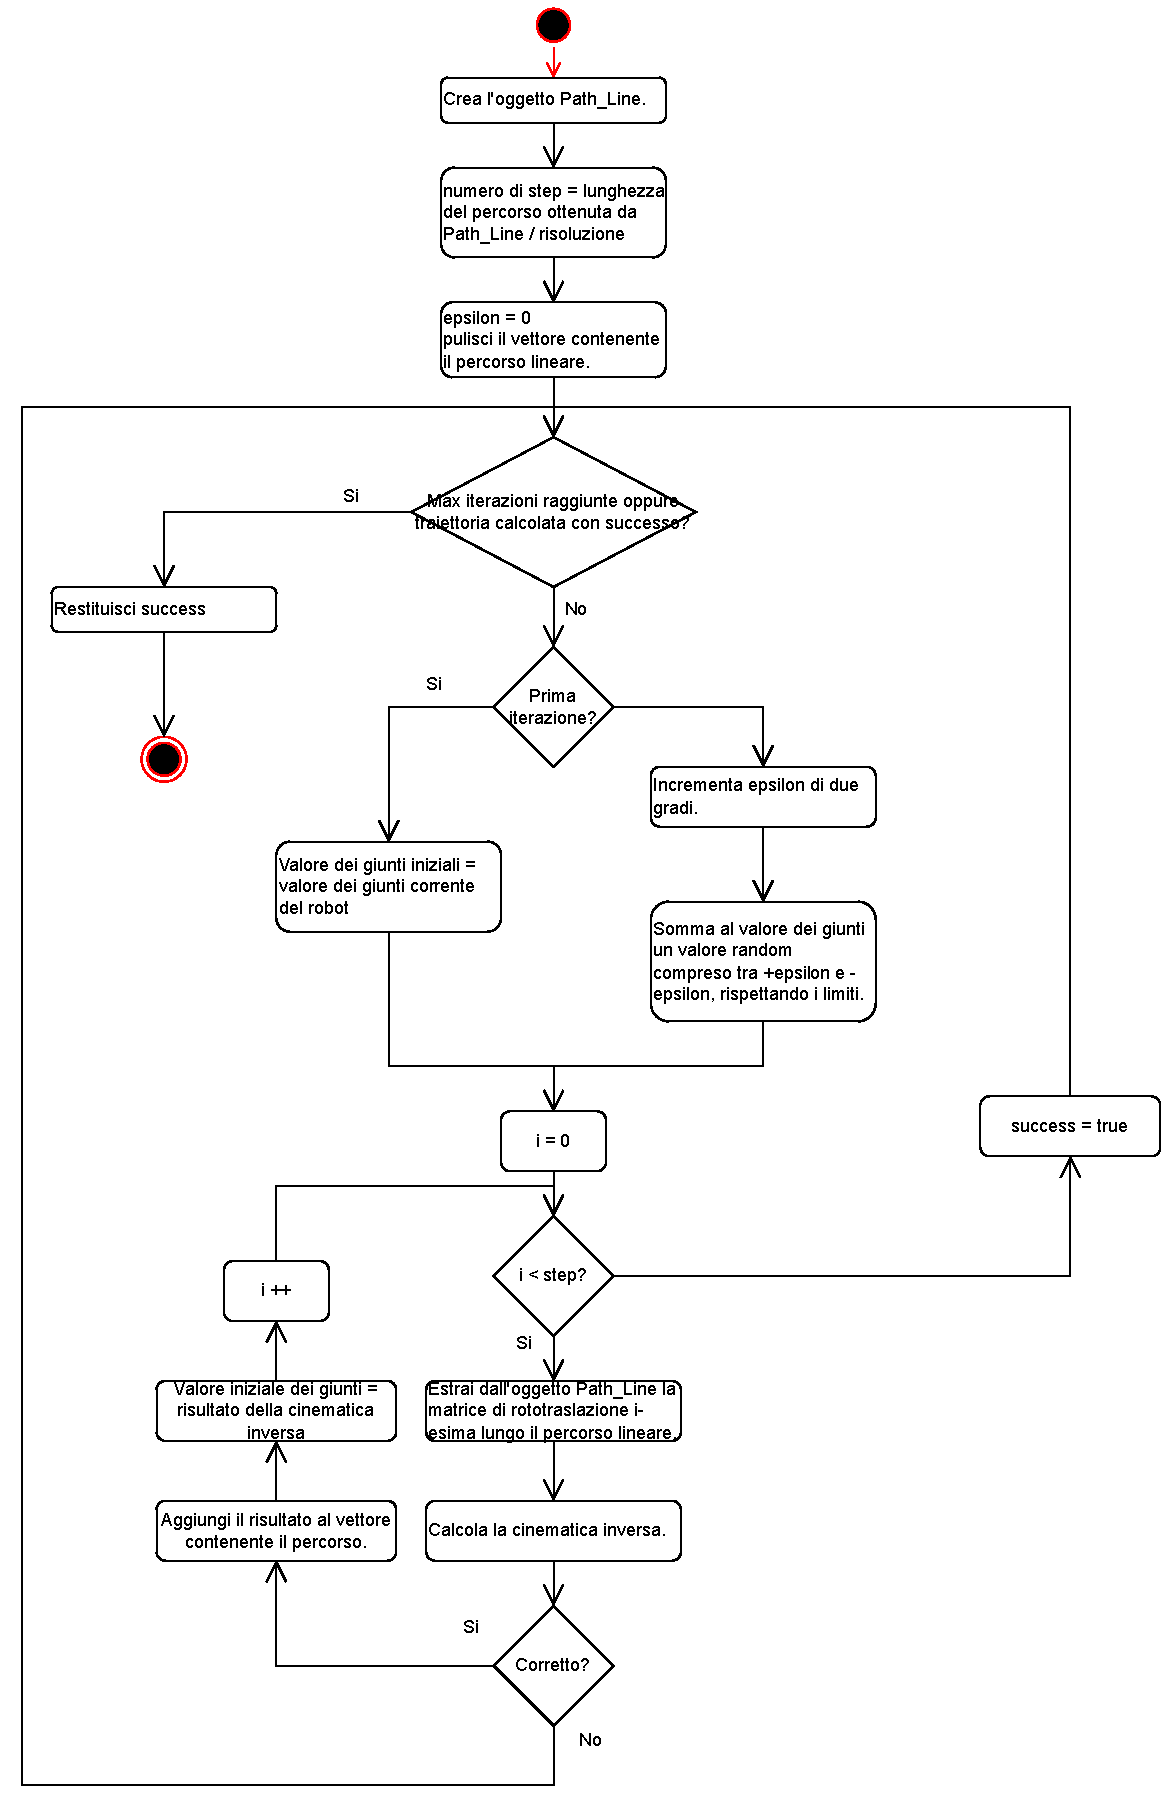
\includegraphics[width=1\linewidth]{./ImageFiles/ComputeLinearTrajectory.drawio.pdf}	\caption{Diagramma di flusso che mostra il funzionamento dell'algoritmo che calcola il percorso lineare.}
	\label{fig:algorithm}
\end{figure}
\clearpage

\section{Componenti: ArmDriver e ToolInput}
La comunicazione con il robot è gestita dal componente \textit{ArmDriver} che implementa due attività: la \textit{JointControlActivity} e la \textit{ToolControlActivity}. Queste due attività vengono inizializzate e registrate nel metodo \texttt{ArmDriver::startup()} della classe \texttt{ArmDriver}. 

L'attività \textit{JointControlActivity} è una \textit{periodic activity}, che riceve una traiettoria dal topic \textit{joint\_trajectory} e pubblica lo stato corrente dei giunti sul topic \textit{joint\_state}. Inoltre, si interfaccia con la \textit{functionality} \texttt{ArmInterface} che si occupa della comunicazione con il nodo ROS integrato nel robot. Quando viene pubblicata una traiettoria, viene chiamata la funzione di callback \texttt{JointControlActivity::jointTrajectoryCallback(VariantActivity* va)}, che si occupa di estrarre ogni punto di passaggio del percorso ricevuto e inviarlo al robot tramite l'interfaccia \texttt{ArmInterface}. 

L'attività \textit{ToolControlActivity} è una \textit{sporadic activity} che riceve la posizione target dell'end-effector sul topic \textit{tool\_command} e lo stato attuale dei giunti sul topic \textit{joint\_state} mentre pubblica la traiettoria calcolata sul topic \textit{joint\_trajectory}. Inoltre, si interfaccia con la \textit{functionality} \texttt{KinematicsInterface} che permette di richiamare le funzioni presenti nel plugin \texttt{PluginArmPRob3Kinematics}. Ogni volta che l'attività riceve lo stato dei giunti dalla \textit{JointControlActivity} li memorizza nella variabile \textit{std::vector\tl double\tr lastJointState}. Invece, quando riceve dal componente \textit{ToolInput} la posizione target dell'end-effector viene richiamata la funzione di callback \texttt{ToolControlActivity::toolCommandCallback (VariantActivity *va)} che si occupa di pubblicare la traiettoria. In particolare, inizialmente viene calcolata la posizione attuale dell'end-effector grazie alla cinematica diretta calcolata a partire dall'ultimo stato dei giunti ricevuto. Se il calcolo va a buon fine e il comando ricevuto richiede il calcolo di una traiettoria lineare, si procede al calcolo del percorso lineare dalla posizione attuale calcolata e la posizione target ricevuta (tramite la funzione \texttt{computeLinearTrajectory}). Se viene calcolato in modo corretto un percorso lineare, si procede alla pubblicazione della traiettoria sul topic \textit{joint\_trajectory}, che sarà poi ricevuta ed eseguita dalla \textit{JointControlActivity}.

Il componente \textit{ToolInput} si occupa invece di inviare all'attività \textit{ToolControlActivity} la posizione target che l'end-effector deve raggiungere e implementa l'attività \textit{ToolInputCommandActivity}.

L'attività \textit{ToolInputCommandActivity} è una \textit{sporadic activity} che si occupa di leggere la proprietà \texttt{ToolEnd} definita nel file di configurazione del componente. Questa proprietà definisce la posizione target dell'end-effector tramite il seguente formato:
\begin{lstlisting}[language=xml]
	<ToolEnd>
		Value>x y z roll pitch yaw</Value>
	</ToolEnd>,
\end{lstlisting}
dove \textit{x, y, z} sono espressi in metri mentre \textit{roll, pitch, yaw} sono espressi in radianti. Una volta letta, la posizione sarà inserita in un \texttt{star::manipulation\_msgs::ToolMotionCommand} e sarà pubblicata sul topic \textit{tool\_command}. Essa verrà ricevuta dall'attività \textit{ToolControlActivity} che procederà al calcolo della traiettoria.